\documentclass{beamer}
\usetheme{owl}           % Use metropolis theme
\newcommand\tab[1][1cm]{\hspace*{#1}}
\title{Overview of Themnothorax decision model (Stephen Pratt \& Mallon et al 2001-2005)}
\date{\today}
\author{Lucas Saldyt}
\institute{Arizona State University}

\usepackage{xcolor}
\usepackage{amsmath}

\makeatletter
\def\mcolor#1#{\@mcolor{#1}}
\def\@mcolor#1#2#3{%
  \protect\leavevmode
  \begingroup
    \color#1{#2}#3%
  \endgroup
}
\makeatother

\newcommand{\annotate}[3]{
\mcolor{#1}{\overbrace{#3}^\text{#2}}
}

\newcommand{\sitem}[1]
{
    \begin{itemize}
        \item #1
    \end{itemize}
}

\bibliographystyle{naturemag}

\definecolor{orange}{HTML}{f7c767}
\definecolor{blue}{HTML}{67E6F7}
\definecolor{green}{HTML}{bdf767}
\definecolor{purple}{HTML}{f467f7}
\definecolor{red}{HTML}{fc4475}

\usepackage{tikz}
\usetikzlibrary{arrows.meta}

\begin{document}
  \maketitle
  \begin{frame}{Introduction}
      \begin{columns}
          \begin{column}{0.5\textwidth}
              \begin{itemize}
                  \item Temnothorax Albipennis prefers to live in rock crevasses, and emigrates frequently.
                  \item Emigration decision behavior is decentralized and self-organizing, and therefore interesting.
              \end{itemize}
          \end{column}
          \begin{column}{0.5\textwidth}
               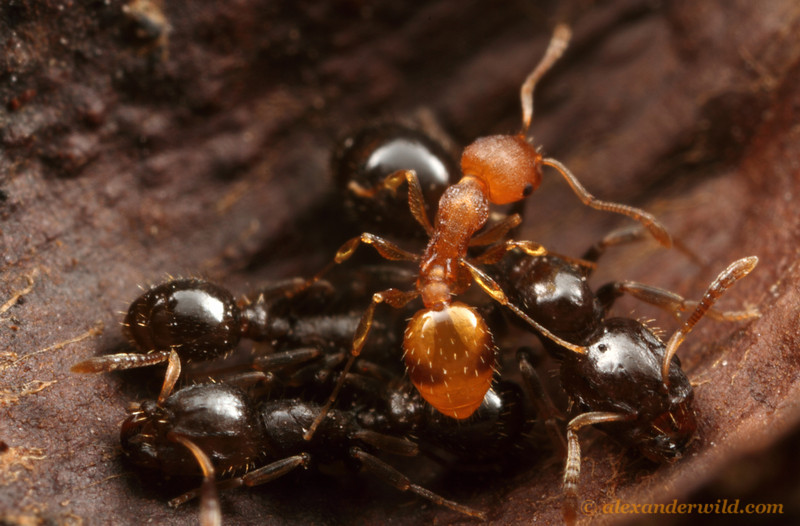
\includegraphics[scale=1.0]{americanus}
          \end{column}
      \end{columns}
  \end{frame}

  \begin{frame}{Research Questions (Mallon 2001)}
      \begin{itemize}
          \item How does small colony size affect decision making?
              \sitem{\mcolor{red}{Graded assessment} affects the colony feedback loop}
          \item What proportion of comparison is by individuals as opposed to at the colony level? 
          \sitem{\mcolor{red}{$86\%, 46\%, 32\%$} for different colonies.}
          \sitem{Direct comparison is \mcolor{red}{not crucial} for choosing the optimal site and therefore the decision is \mcolor{red}{decentralized}}
          \item What physical observations act as cues for behavior? 
              \sitem{\mcolor{red}{Nestmate interaction rate} for estimation of colony/environment state}
      \end{itemize}
  \end{frame}

  \begin{frame}{Research Questions (Pratt 2002)}
      \begin{itemize}
          \item What is the purpose of multiple recruitment mechanisms? (Pratt 2002, 2005)
              \sitem{Tandem runs allow route learning and pheromone depositing}
              \sitem{\mcolor{red}{Graded commitment} allows error-correction and optimal decision making.}
              \sitem{Recruitment \mcolor{red}{accelerates} when transport begins ($3x$ speed)}
          \item How do individuals choose between recruitment mechanisms? (Pratt 2005)
              \sitem{Transports preffered once \mcolor{red}{quorum} is met}
          \item How does decentralization happen without direct comparison? (Pratt 2005)
              \sitem{Recruit to better sites faster $\rightarrow$ \mcolor{red}{positive feedback}}
      \end{itemize}
  \end{frame}

  \begin{frame}{Research Questions (Pratt 2002)}
      \begin{itemize}
          \item What is the purpose of the reverse-tandem mechanism?
              \sitem{Stimulate transport by idle workers}
              \sitem{Fix nest-splitting that may occur in nature (More likely)}
          \item What is the purpose of the quorum requirement?
              \sitem{Assists optimal choice without direct comparison}
              \sitem{Mistake correction mechanism}
              \sitem{Minimize colony splitting}
              \sitem{Selection of an individual ant's ``home`` nest}
          \item How is quorum detected?
              \sitem{Ants likely use \mcolor{red}{rate estimation} rather than literal counting}
          \item \mcolor{red}{\em{Important parts of the decision process occur at the individual level}}
      \end{itemize}
  \end{frame}

  \begin{frame}{2002 Model Overview}
      Models colony of $N$ ants, where proportion $p$ are active. \\
      $M$ sites (in practice $~2-12$ sites). \\
      Four population classes: 
      \begin{itemize}
          \item $S$: Searching (At destroyed nest or between nests) \mcolor{red}{(Initially $Np$)}
          \item $A_i$: Assessing a nest $i$ \mcolor{red}{(Initially 0)}
          \item $R_i$: Recruiting to a nest $i$ \mcolor{red}{(Initially 0)}
          \item $P_i$: The passive population at nest i \mcolor{red}{($P_0 = N(1-p), P_i = 0$)}
      \end{itemize}
  \end{frame}


  \begin{frame}{Overview of Pratt 2002 Equations (Colors showing flow of ant population)}
      \Large
      \begin{equation}
      \begin{aligned}
          & \frac{dS}{dt} = - \sum_{j=1}^M \mcolor{orange}{u_jS} - \sum_{j=1}^M \mcolor{purple}{\lambda_jI(R_j, S)} \\
          & \frac{dA_i}{dt} = \mcolor{orange}{u_iS} + \mcolor{purple}{\lambda_jI(R_j, S)} + \sum_{j \neq i}^M \mcolor{blue}{(\rho_{ji}A_j - \rho_{ij}A_i)} - \mcolor{green}{k_iA_i} \\
          & \frac{dR_i}{dt} = \mcolor{green}{k_iA_i} + \sum_{j \neq i}^M \mcolor{blue}{(\rho_{ji}R_j - \rho_{ij}R_i)} \\
          & \frac{dP_i}{dt} = \annotate{red}{Causes overflow if unchecked}{\phi_iJ(R_i, P_0)} - \annotate{white}{Fix: Subtract moved ants}{\phi_{dest}J(R_{dest},P_0)}
      \end{aligned}
      \end{equation}
  \end{frame}

  \begin{frame}{Search population}
      \Large
      \begin{multline}
      \frac{dS}{dt} = - \sum_{j=1}^M \annotate{orange}{Rate of finding nest $j$}{u_j}*S \\  
      - \sum_{j=1}^M \annotate{purple}{Ants led by tandem run}{\lambda_jI(R_j, S)} 
      \end{multline}
  \end{frame}
  \begin{frame}{Assessment population}
      \Large
      \begin{multline}
      \frac{dA_i}{dt} = \annotate{orange}{Ants that find nest $i$ and begin assessing it}{u_iS} \\ 
      + \annotate{purple}{Ants led by tandem run}{\lambda_jI(R_j, S)} \\
      + \sum_{j \neq i}^M \annotate{blue}{Ants encountering alternative sites}{(\rho_{ji}A_j - \rho_{ij}A_i)} \\ 
      - \annotate{green}{Ants that become recruiters}{k_iA_i} \\
      \end{multline}
  \end{frame}
  \begin{frame}{Recruitment population}
      \Large
      \begin{multline}
          \frac{dR_i}{dt} = \annotate{green}{Ants that become recruiters}{k_iA_i} \\
          + \sum_{j \neq i}^M \annotate{blue}{Ants encountering alternative sites}{(\rho_{ji}R_j - \rho_{ij}R_i)}
      \end{multline}
  \end{frame}
  \begin{frame}{Passive population}
      \Large
      \begin{equation}
          \frac{dP_i}{dt} = \underbrace{\annotate{red}{Per capita transport rate}{\phi_i} * \annotate{red}{Quorum requirement}{J(R_i, P_0)}}_\text{Carried passive ants}
      \end{equation}
  \end{frame}
  \begin{frame}{Auxilary Functions}
      \Large
      Tandem/Carrying switching rule:
      \begin{equation}
          I(R_i, S) = 
          \begin{cases}
              & R_i,  \text{ if } \annotate{red}{Recruiters below threshold}{R_i < T} \\
              &       \text{     and } \annotate{red}{While there are recruitable ants}{S > 0}\\
              & 0, \text{ otherwise}
          \end{cases}
      \end{equation}
  \end{frame}

  \begin{frame}{Auxilary Functions}
      \Large
      Quorum rule:
      \begin{equation}
          J(R_i, P_0) = 
          \begin{cases}
              & 0,  \text{ if } \annotate{red}{Recruiters below threshold}{R_i < T} \\  
              &     \text{     or } \annotate{red}{Edge case: migration has finished}{P_0 = 0}\\
              & R_i, \text{ otherwise}
          \end{cases}
      \end{equation}
  \end{frame}

  \begin{frame}{Assumptions}
      \begin{itemize}
          \item Ants always move exclusively out of the searching state
          \item Finding/Recruitment/Switching/Conversion rates are all constant per nest
          \item Requires detailed parameter estimation
      \end{itemize}
  \end{frame}

  \begin{frame}{Diagram of ODE model (Pratt 2002)}
       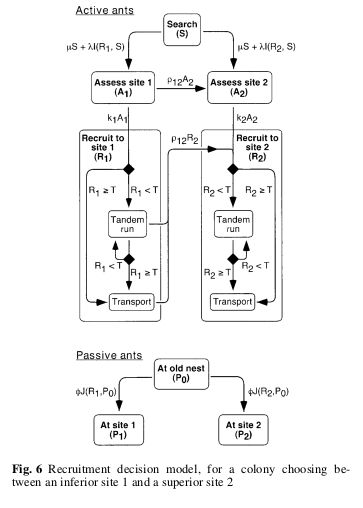
\includegraphics[scale=1.0]{diagram}
  \end{frame}

  \begin{frame}{The agent based model (Pratt 2005)}
       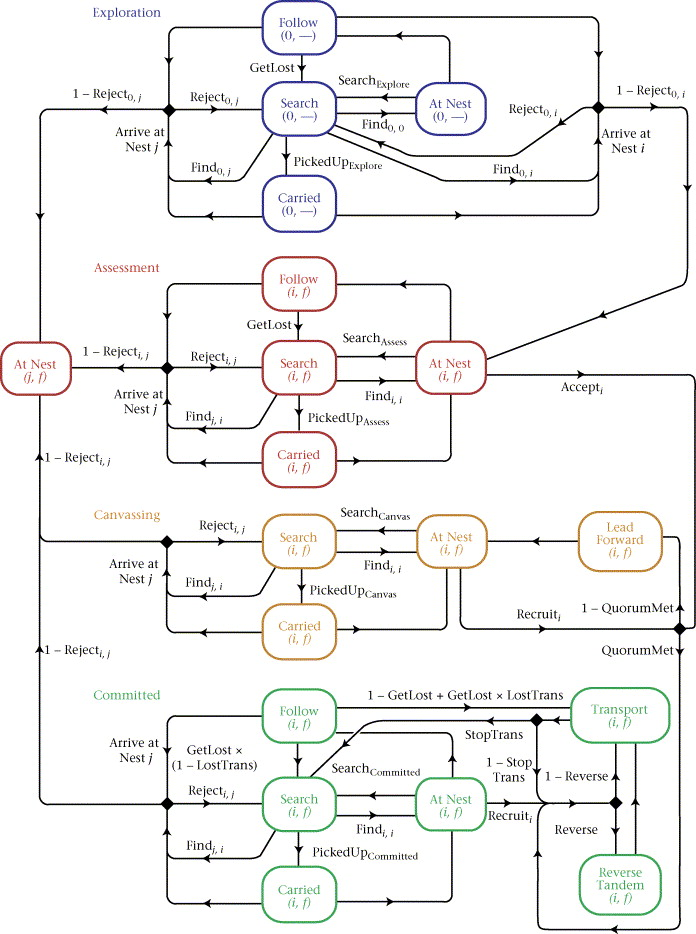
\includegraphics[scale=1.6]{agent}
  \end{frame}

  \begin{frame}{Important differences between the models (In order of subjective importance)}
      \begin{itemize}
          \item Ants remember their ``home`` nest.
          \item Commitment level is separated from individual actions 
              \sitem{(i.e. an ant can follow even in the committed state)}
              \sitem{Also allows for further parameterization}
          \item Intentionally makes the model more brittle so that it can be further tested empirically. 
              \sitem{A general model is potentially harder to disprove}
          \item Adds a simple ``at-nest`` action 
          \item Minute differences (potential for ants to get lost)
      \end{itemize}
  \end{frame}

%%   \begin{frame}{Proposed Ordinary Differential Equation Model}
%% 
%%   The proposed model begins with an improved set of ordinary differential equations, based on Pratt 2002.
%%   It contains equations for five separate populations: 
%%   \begin{itemize}
%%       \item $S$, the searching population (not at any nest)
%%       \item $A_i$, the assessing population at nest $i$
%%       \item $L_i$, the leading (forward-tandem-running) population at nest $i$
%%       \item $C_i$, the carrying (transport) population at nest $i$
%%       \item $P_i$, the passive population at nest $i$. 
%%   \end{itemize}
%%   The model focuses on the following:
%%   \begin{itemize}
%%       \item Splitting the $R_i$ population from S. Pratt 2002 into the $L_i$ and $C_i$ populations.
%%       \item Replacing the two switching equations $I()$ and $J()$ with dynamics switching between $L_i$ and $C_i$ based on a single switching equation $Q()$.
%%       \item Fixing unchecked growth in the original $P_i$ equations.
%%       \item Allowing transport of various passive populations, which will allow a split passive population to be fixed.
%%       \item Replacing switching in $A_i$ and $R_i$ with transitions to searching population. This reflects updates in S.Pratt 2005 and Granovskiy 2012 agent-based models.
%%       \item Adding transportation of the active searching population (but not the assessing, leading, or carrying populations).
%%   \end{itemize}
%% 
%%   Given $N$ ants, where proportion $p$ are active, the initial states are the following:
%%   \begin{itemize}
%%       \item $S = pN$
%%       \item $P_0 = (1-p)N$ 
%%       \item $A_i, L_i, C_i, P_i = 0$ 
%%   \end{itemize}
%% 
%%   The original model used the following parameters:\\
%% 
%% \begin{tabular}{ l | r }
%%     \hline
%%   $\mu_i$     & Likelihood of finding nest $i$\\
%%   $\lambda_i$ & Proportion led by leaders to $i$\\
%%   $\rho_{ij}$ & Switching rates between nests $i$ and $j$\\
%%   $k_i$       & Acceptance probability for nest $i$\\
%%   $\phi_i$    & Rate for carrying passive ants to nest $i$\\
%%     \hline
%% \end{tabular} \\
%% 
%% The updated model builds on this list, but renames old parameters to make them more intuitive: \\
%% 
%% \begin{tabular}{ l | c | r }
%%     \hline
%%   Name          & 2002        & Description (units = rate)\\ \hline
%%   $\phi_i$      & $\mu_i$     & Finding nest $i$\\
%%   $\lambda_i$   & $\lambda_i$ & Led by leaders to $i$\\
%%   T             & T           & Threshold (positive integer)\\
%%   $\alpha_i$    & $k_i$       & Assessors who accept nest $i$\\ \hline
%%   $\tau_{Pi}$   & $\phi_i$    & Passive ants are transported to $i$\\
%%   \end{frame}

  \begin{frame}{Bibliography}
      \bibliography{sources/insects,sources/brains,sources/ant_system,sources/networks,sources/misc}
  \end{frame}

\end{document}
